
\section{Design}

This section presents the design of {\name}, including the overall architecture,
the data model, and the protocols for the {\em put}, {\em get} and {\em delete} operations.

\subsection{Overview and challenges}

\begin{figure}[tp]
\centering
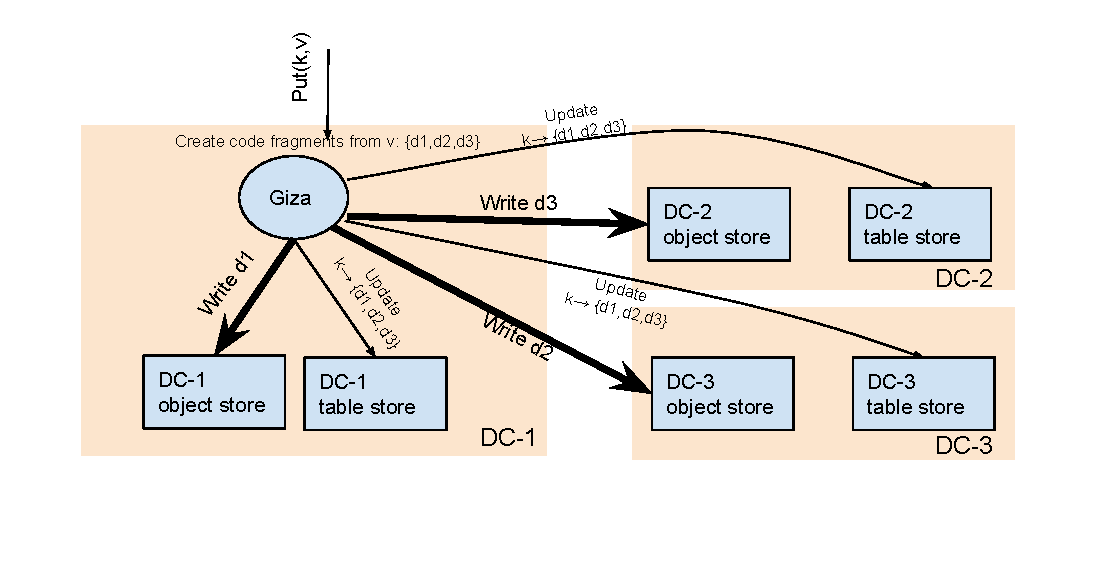
\includegraphics[width=0.5\textwidth]{fig/Giza}
\caption{Giza architecture\label{fig:arch}}
\end{figure}

\paragraph{Architecture}
{\name} is a global-scale cloud storage system 
that spans across many data centers in the world.
It stores mutable, versioned objects.
Figure~\ref{fig:arch} shows the architecture of \name. 
\name separates data path from meta-data path.
On the data path, \name splits and encodes the object into data and parity fragments.
Each fragment is uniquely named by its content hash
and stored in a different DC.
Updates to the object create new versions.
The version numbers, together with the hashes of the coded fragments in each version,
consist of the meta-data of the object.
On the meta-data path, \name replicates the meta-data across the data centers.

We implement \name by layering on top of an existing cloud storage infrastructure. This 
provides two advantages.  First, doing so allows the rapid development of \name by re-using 
mature, deployed systems.  Second, it simplifies the failure recovery and 
the deployment of \name, as \name nodes are completely stateless and can be
readily integrated with the rest of the stateless cloud storage front-ends.

%Existing cloud storage systems have redundancy within a single data center, but are not geo-replicated.  Thus, \name must explicitly provide cross data center redundancy through coding and replication.
To write the object,
{\name} stores the coded fragments in different data centers in {\em cloud blob stores},
such as Azure Blob, or AWS S3.
Additionally, \name replicates the object's meta-data across multiple data centers 
and stores the metadata in {\em cloud tables}, such as Azure Table, or AWS DynamoDB. 
The number of the coded fragments, and thus the set of data centers
storing the data object, is configurable during the account setup depending on the user desired tradeoff on
durability vs. cost.
%The number of data centers to replicate the meta-data is fixed at 3.

%blob service as building blocks, to store metadata and data respectively. This evolutional
%design allows {\name} to minimize footprint of new code. In fact, {\name} merely needs to replace the previous front-end
%module. With {\name} deployed, the user request comes in to the new frontend, where the new
%{\name} service will translate the user requests into a few metadata operations and data operations.
%
%In {\name}, both metadata and data are synchronously duplicated across different
%datacenters in order to tolerate datacenter failures. What is different between metadata
%and data is, metadata is fully replicated across a (usually smaller) set of datacenters using
%a tailored Fast-Paxos algorithm, persistent in the table service in each datacenter, thus
%tolerating a minority of failures; On the other hand, data in user request is encoded to
%a configurable number of fragments and shipped to a (usually larger) set of datacenters,
%persistent in the blob storage service. We refer the former as metadata path and the latter
%as data path.


\paragraph{Technical challenges}
Giza names each coded fragments by their content hashes.
As a result, each coded fragments is immutable, as updating the object would result in completely different fragments and hashes.
Hence, storing immutable fragments in the cloud blob stores makes the data path straightforward and greatly simplified. 

On the other hand, the metadata path of Giza is subtle.
In designing \name, we address three main technical challenges involving the metadata path.
\begin{enumerate}

\item {\it Building a strongly consistent, geo-replicated meta-data storage out of existing 
single-DC cloud tables.}
There are existing solutions, such as Cassandra and CockcoarchDB,
that offer strongly consistent, geo-replicated storage systems.
Giza chooses not to adopt the existing solutions because
1) it is desirable to make \name nodes stateless and keep all data and meta-data
in existing cloud storage infrastructure;
2) it is preferable to implement protocols best suited for our targeted workloads,
so as to achieve optimal latency.
Indeed, Giza ensures strong consistency by implementing the Paxos consensus protocol.
The trick is to implement Paxos using existing cloud storage APIs and achieve 
optimal latency in the cross-DC setting.

\item {\it Jointly optimizing the data and meta-data paths to achieve a single
cross-DC round trip for read/write operations.}
A naive approach would execute the data and metadata path sequentially:
a \name node completes the data path, write out the blob first before starting on the meta-data path.
While doing so guarantees that data is durably written at multiple DCs
before it becomes externally visible, each write operation requires at least two cross-DC round trips.
Similarly, a naive approach for read operation would take the first cross-DC round trip to retrieve the metadata
and then the second round trip to retrieve the data.
Can \name combine the data and metadata path operations to achieve a single cross-DC round trip for both read and write?

\item {\it Performing garbage collection efficiently and promptly.} 
\ch{Revisit later.}
When data is over-written and deleted, \name must remove obsolete data and/or meta-data from
the underlying cloud storage. Also, when a data writes fail, \name may left partially written data, which need to be
garbage collected.  
This is non-trivial because \name's garbage 
collection mechanism must be able to handle data center failures while ensuring data 
consistency and durability.

\end{enumerate}

%The separation of metadata path and datapath bring in the challenge that the consistency level
%could be violated with brutal yet flawed merge of the two. Our protocols described in later
%sections will guarantee the metadata path and data path together (especially when they are
%fully concurrent) will still provide a strong consistency insurance.
%


% A typical giza architecture for a data center includes the giza nodes, the Azure Blob Storage, and the Azure Table Storage. The giza nodes are the processing units of the Giza architecture and manages the data and the metadata. Furthermore the giza nodes participate in paxos rounds as coordinators. Figure 1 illustrates the architecture of Giza. Giza separates data from metadata and handles them on different paths. The data path is responsible for encoding the data and sending the data fragments across data centers. Each data fragment is stored in the corresponding DC’s Azure Blob Storage. The metadata path is responsible for storing the latest version of the data and the location of its data fragments. Giza uses a variant of the Paxos state machine replication (SMR) to maintain consistency of the metadata where each metadata server maintains a local copy of the replicated log. The replicated log is stored in the Azure Table Storage.

\subsection{Implementing Paxos using Cloud Storage APIs}

On the meta-data path, \name implements a Paxos consensus protocol to serialize the operations on each data object.
More specifically, it implements Paxos on top of existing cloud tables, such as Azure Table, or AWS DynamoDB.

\subsubsection{Paxos and Fast Paxos: A Brief Primer}

The Paxos algorithm provides a mechanism to reach consensus among a set of {\em acceptors} and one or more {\em proposers}. Each proposer initiates a Paxos voting process by first picking a distinguished {\em ballot}. All ballots are unique and can be compared to each other. The proposer send requests to the acceptors, and associate each request with a proposal value. Each acceptor decides whether to accept a request based on its own state. The proposal value is {\em committed} when it is accepted by a {\em quorum} of the acceptors. The acceptors update their states when a request or value is accepted.

In our implementation, each Giza node is a proposer. The acceptors in Paxos are typically active processors, which are capable of comparing the ballot of an incoming request with its own state and deciding whether to accept the request. In Giza, we implement the acceptors using the cloud table storage. Comparing the ballot and accepting the request is implemented via {\em atomic conditional update} to the table.

Paxos takes two {\em phases} to reach consensus, where {\em phase} $1$ prepares a ballot and {\em phase} $2$ accepts a value. Since each phase takes one round trip, applying Paxos in Giza results in two cross-DC round trips for metadata writes~\footnote{Typical Paxos optimization elects a distinguished leader. The leader executes {\em phase} $1$ in advance and only takes one round trip in {\em phase} $2$ to reach consensus. This, however, requires relaying all updates through the leader. In the cross-DC scenario, it takes one cross-DC round trip to relay updates originating from non-leader DCs. Therefore, these updates still take two cross-DC round trips to commit.}.

Fast Paxos is a version of Paxos designed to optimize the performance over cross-DC acceptors. It employs two types of rounds: fast round and classic round. A fast round sends a PreAccept request and takes a single round trip to reach consensus. A classic round resembles the two phases in Paxos and takes two round trips.
The fast round in Fast Paxos demands a larger quorum than that in Paxos. Consider a case with $3$ acceptors. Paxos is able to reach consensus with 2 out of the 3 acceptors (quorum size of 2). In comparison, Fast Paxos only reaches consensus with all the 3 acceptors (quorum size of 3).

In Giza, the success of the data path requires multiple data centers to be online to make progress, it turns out easy to satisfy the demand of a larger quorum, and suites the implementation need in Fast Paxos. E.g., Giza requires at least 3 data centers to stripe the coded fragments (with $2 + 1$ erasure coding). Hence, the data path won't succeed unless there are at least 3 data centers available, which makes it easy to satisfy the larger quorum requirement.

Giza implements both Paxos and Fast Paxos. In the below description, we focus on Fast Paxos and skip the details regarding Paxos.
%Hence, the most optimized metadata path in Giza implements Fast Paxos, as detailed next.

\begin{figure}[tp]
\centering
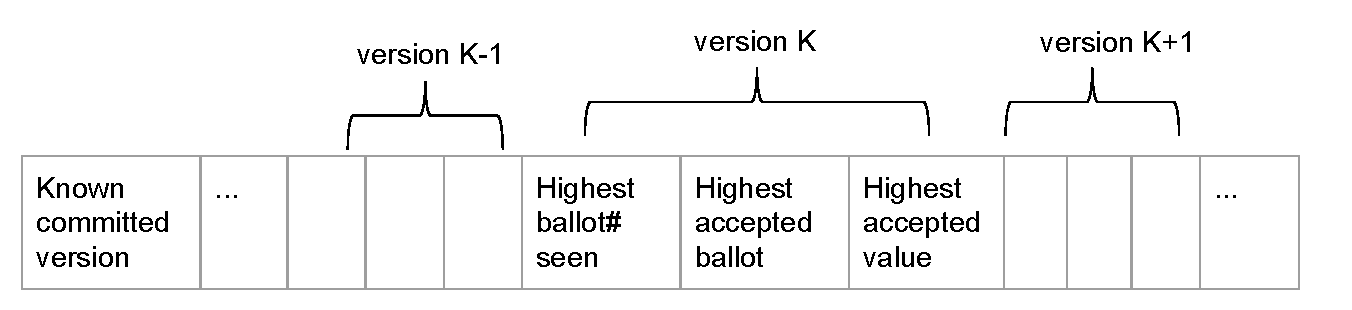
\includegraphics[width=0.5\textwidth]{fig/Giza_Metadata}
\caption{For each object, \name stores the Paxos protocol state and the object meta-data 
in a single row in the underlying cloud table.\label{fig:metadata}}
\end{figure}

\subsubsection{Meta-data Storage Layout}

%\name implements the Paxos consensus protocol to serialize the operations on each data object.
To implement the Paxos consensus protocol,
\name needs to persist the Paxos states in addition to the metadata for the object.
{\name} conveniently stores the Paxos states together with the metadata in the cloud table,
one table row per object, with a dynamic number of columns. The layout of each table row is
shown in Figure~\ref{fig:metadata}.

Each object may have multiple versions.
The versions are represented by consecutive natural numbers, starting from $1$.
A \name write operation leads to a new version of the object.
For each version, Giza invokes a separate Paxos instance to ensure consistency
in the event of races among multiple writers and failures.
The states of all the Paxos instances are stored in the same table row,
as part of the metadata for the data object.
Specifically, the meta-data contains a triplet of columns for each version of the object
(Figure~\ref{fig:metadata}).
%The triplet includes {\tt highest\_proposal\_seen}, {\tt highest\_accepted\_proposal}, and {\tt highest\_accepted\_value}.
The triplet includes {\tt highest ballot seen} and {\tt highest accepted ballot},
for recording the states of each Paxos instance.
The triplet also includes {\tt highest accepted value},
which contains the meta-data information, including the erasure coding scheme,
the name of each coded fragment, whether it is one of the original or parity fragments,
and which DC the fragment is stored at.

{\name} additionally maintains a set of {\tt known committed versions} 
for all those that have been committed by Paxos. As will become clear later,
this set provides a hint to facilitate both write and read operations.
It is a hint in the sense that newly committed versions are added to the set asynchronously,
or beyond the critical path of write operations.
Hence, while all the version numbers in the set are guaranteed to have been committed,
the latest committed version number might yet have to be included.

\subsubsection{Meta-data Write - Common Case}

The metadata path begins with choosing a proper new version number to run the Fast Paxos~\cite{fastpaxos} algorithm.
Since version numbers are consecutive, the new version needs to be next to the most recently committed version.
While it is safe to use an outdated version
(in which case the {\name} node will later realize its mistake and retry with a higher version number),
it is unsafe to choose a higher one and results in non-consecutive versions.
The {\name} node identifies the proper version in an optimistic fashion.
Specifically, it reads {\tt known committed versions} from the table in its local DC,
then uses the next higher number as the chosen version number to invoke the corresponding Fast Paxos instance.

With the version number chosen, the {\name} node replicates a PreAccept request
to the tables in all the DCs.
Each request is an {\em atomic conditional update} to the corresponding table in a single DC.
If there are no competing requests on the same version, the PreAccept request will succeed in updating the table row.
Otherwise, the PreAccept request will be rejected by the table and leave the table row unchanged.
Section~\ref{sec:implementation} illustrates how atomic conditional update is implemented leveraging existing cloud APIs.

Whenever the {\name} node receives a {\em fast quorum} of positive PreAccept responses,
the corresponding version is considered to have been committed.
The {\name} node asynchronously replicates a Commit confirmation to all the DCs to update 
the set of {\tt known committed versions} to include the recently committed version.
The Commit confirmation is again an atomic conditional update,
which only succeeds if the version number is not yet included in the current set.

Since the Commit confirmation is completed asynchronously,
the critical path only involves the PreAccept request and response.
Hence, the above described metadata write involves only one cross-DC round trip 
and is referred to as the {\em fast path}.  When there is no
contention, the fast path always succeeds.

\subsubsection{Meta-data Write with Contention}

In the case of contention, the fast path may not succeed, i.e. the {\name} node
cannot collect a fast quorum of positive PreAccept responses. The contention
may come from concurrent updates to the same version, or a {\name} node trying
to recover from failures by re-committing the same or a different value to an
ongoing version.  In this case, {\name} enters what is referred to as a
\emph{slow path} to perform classic Paxos in order to guarantee safety in case of
contention.

On the slow path, the {\name} node first picks a distinguished ballot number
and then replicates a Prepare request to write the ballot to all the metadata
tables and wait for a majority of responses.
The Prepare request is a conditional update operation.
The operation succeeds only if the {\tt highest ballot seen} is no more than 
the ballot in the Prepare request.
The operation also returns the entire row as a result.

Upon collecting a majority of successful replies, the {\name} node needs to pick a value to commit.
The rule for picking the value is categorized into three cases.
In case 1, Giza looks for the highest accepted ballot in the replies.
If there is one, the value from the reply is picked.
In case 2, the replies contain no accepted value, but rather pre-accepted values.
Giza picks the pre-accepted value that appears more than others (if any) from the replies.
Both case 1 and 2 imply the possibility of an ongoing Paxos instance,
so Giza picks the value so as to complete the Paxos instance first.
It then starts with a new version and follows the fast path to commit its current metadata.
In case 3, there is neither pre-accepted nor accepted value,
which implies no real impact from contention.
Giza picks its current metadata as the value and proceeds to next steps.

Once the {\name} node picks a value, it replicates an Accept request to all the metadata tables.
The accept request is again an atomic conditional update; it succeeds in writing {\tt
highest accepted ballot} and {\tt highest accepted value} if neither {\tt
highest ballot seen} and {\tt highest accepted ballot} is larger.
As soon as a majority of Accept requests succeed, the \name node considers the
corresponding meta-data write completed and sends acknowledgment to clients.
Additionally, a Commit confirmation is replicated in the background, as described before.

\subsubsection{Metadata Read}

To get the metadata of the \emph{latest} object version,
it is insufficient for Giza to only read the corresponding metadata table row from its local DC.
This is because the local DC might not be part of the majority quorum that has accepted the latest version.
To ensure correctness, Giza needs to read the metadata rows from more than one DC.

In the common case,
{\tt known committed versions} is already updated and includes the latest committed version (say version $k$).
The metadata table row from the local DC obtains version $k$.
And the metadata table row from a non-local DC confirms the lack of higher committed versions than $k$.
Hence, in the case that the metadata is replicated to 3 DCs,
the metadata from 2 DCs (one local and one non-local) leads to a decisive conclusion that version $k$ is the latest committed version.
It is therefore safe for the Giza node to return version $k$ to clients.

In general, the \name node reads the metadata table rows from all the DCs.
Whenever a majority rows have matching {\tt known committed versions}
and have not accepted any value for a higher version, 
the \name node returns the metadata of the highest committed version.

If unfortunately the replies contain a higher version with accepted value while not included in {\tt known committed versions},
the \name node needs to follow a slow path similar to the one in the write operation.
This is to confirm whether the higher version has indeed been committed,
despite that the version is not included in {\tt known committed versions} and the metadata tables in certain DCs may have missed the quorum.

%This is because it could possibly be considered committed once before. After it succeed in the slow path, the {\name} node needs to re-launch the datapath to retrive the data fragments of the newer version and abandon the old ones. This serialized metadata and datapath case typically happens when there is concurrent read and write on the same object, which is rare in our workload.

%\sm{ Hi Daniel, just want to confirm, is this what you do now? Only one accepted in higher version will invalidate the optimistic read}

% continue to design_part2.tex
